% Created 2019-04-07 Sun 22:03
\documentclass[abstract=off,oneside]{scrreprt}
\usepackage[utf8]{inputenc}
\usepackage[T1]{fontenc}
\usepackage{fixltx2e}
\usepackage{graphicx}
\usepackage{longtable}
\usepackage{float}
\usepackage{wrapfig}
\usepackage{rotating}
\usepackage[normalem]{ulem}
\usepackage{amsmath}
\usepackage{textcomp}
\usepackage{marvosym}
\usepackage{wasysym}
\usepackage{amssymb}
\usepackage{hyperref}
\tolerance=1000
\usepackage{caption}
\usepackage{minted}
\author{Thomas Aven}
\date{\today}
\title{TDT4230 - Graphics and Visualization \large \\~\\ Final Project}
\hypersetup{
  pdfkeywords={},
  pdfsubject={},
  pdfcreator={Emacs 25.2.2 (Org mode 8.2.10)}}
\begin{document}

\maketitle

\section*{Introduction}
\label{sec-1}
I've been interested in the world of ray marching for a while, in
particular the fantastic work of Inigo Quilez (found \href{https://iquilezles.org/www/index.htm}{here}). His blog
explains an enormous amount of techniques to create unbelievable
procedural scenes, using only a fragment shader. Most of these shaders
are hosted at Shadertoy.com, which is an online tool for sharing
shaders with WebGL. Code from other shaders I have been inspired by
are all credited in comments in the source code.
\\\\
My primary goal for this project thus became to create interesting
fragment shaders. This means that the only thing I'm allowed to pass
into the vertex shader is a \emph{single quad} that covers the
entire screen -- all the fragment shader has to work with is
\verb~gl_FragCoord~ (with some exceptions, more on that later).
\\\\
For this report I will go through the process step by step, from the
baby steps required to render a simple sphere, to the final leaps that
render a realistic looking scene. There are quite a few illustratory
images, which reside in the appendix, with links back and forth to
make the reading bearable. Limitations with the techniques, as well as
problems encountered will be pointed out along the way.

\section*{Building the project}
\label{sec-2}
The project uses CMake for the building process, as is required for
the assignment. I've also taken the liberty of adding three libraries
to use sound: OpenAL Soft , freealut and FFTW. OpenAL and freealut are
added as submodules with Git, while FFTW is added as an external
project in CMake, which fetches a tarball online, then extracts and
builds the library. Building thus takes a little while, but it's not
too painful. This has been tested with the package repositories found
in Ubuntu 18.04 and Debian Stretch, and should hopefully work right
out of the box.

\section*{Ray Marching}
\label{sec-3}
Now -- what is this ray marching thing? In the world of \emph{ray casting},
it is common to be familiar with \emph{ray tracing} to compute the
intersections of a light ray with surfaces. \emph{Ray marching} may be used
within such a ray tracing method, as it is a specific algorithm for
this purpose. Using ray marching in combination with something that's
called \emph{signed distance functions} can make extraordinary scenes from
infinitesimal binary executables, as all that's required are the
underlying mathematical formulas.
\\\\
A signed distance function, let's say a sphere centered at the origin,
$f(x, y, z) = \sqrt{x^2 + y^2 + z^2} - 1$, for this example, can be
used to determine whether a point is inside or outside an object, as
well as the distance to the object if it is outside. This is in
contrast to more well known ray tracing implementations that have to
check for intersections with quite a lot of primitives (like
triangles).
\\\\
It's time to explain the workings of the method. In \verb~simple.frag~,
there is a function, \verb~sd_sphere~, that takes a point and a radius as
arguments, and returns the distance to its perimeter. Below are two
illustrations I have found to explain the method the best.
\\\\
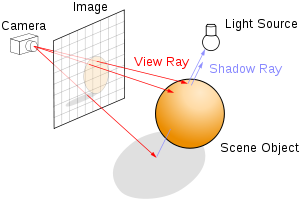
\includegraphics[width=0.45\textwidth]{./img/raytrace.png}
$\hspace{35pt}$
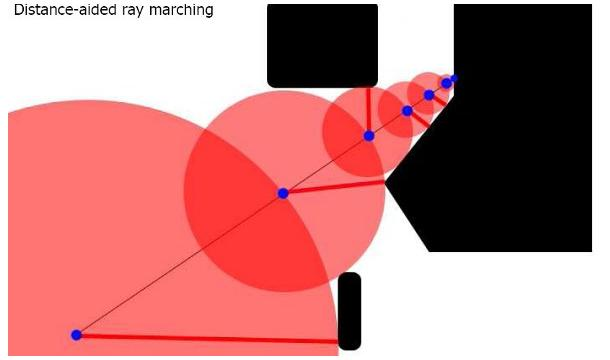
\includegraphics[width=0.45\textwidth]{./img/sphere_tracing.jpg}
\\\\
The \href{http://jamie-wong.com/images/16-07-11/raytrace.png}{left} image shows how rays are traced from a camera. The \href{http://hugi.scene.org/online/hugi37/sphere_tracing.jpg}{right}
image illustrates how the iterative steps are taken by the ray
marching algorithm according to the distance to the object closest to
the current point.

\section*{Humble beginnings}
\label{sec-4}
\label{sec:beginnings}
Let's put our new knowledge to a test -- the execution of the ray
marching algorithm is found in any of the \verb~trace_<object>~
functions. A simple rendering of a sphere with some simple phong
shading is shown in \hyperref[fig:simplesphere]{this image}. Spheres are just the beginning; we
have SDFs for a wide range of shapes: \href{https://iquilezles.org/www/articles/distfunctions/distfunctions.htm}{link}.

\section*{Setting the stage}
\label{sec-5}
\label{sec:creatingascene}
So we have a method of rendering a single object, in this case a
sphere. How do we go about turning this into a complex scene? The
first trick we will pull out of our sleeve is intersections and
unions. If we compute the distance to more than one object, and then
do \verb~max~ (intersect) or \verb~min~ (union) between them, we can have
multiple objects in our scene. The technique can be seen in action
\hyperref[fig:union]{here}. A problem I encountered at this stage was using GLSL
effictively. I practically gave up on optimization, but most of all I
was missing the ability to pass around function pointers for distance
functions (which could perhaps be done with \verb~switch~ statements
anyway, as I'm already murdering the performance with all the
conditionals).

\section*{Shadows}
\label{sec-6}
\label{sec:shadows} An advantage of signed distance functions is that they
provide us with global information. Given a point on a surface in a
scene, we can fairly easily explore our surroundings -- we just have
to recalculate the SDF with new points. For shadowing, we simply
follow what's called a \emph{shadow ray} from the surface point towards the
position of a given light. If it intersects some other object on the
way, the light will not contribute to the illumination. We can also
put areas that are \emph{almost} within the shadow under penumbra by
checking how close we are to intersecting objects on the
way. \hyperref[fig:penumbra]{Illustration}. This perhaps the most pressing advantage of ray
tracing in general: effects such as shadows and reflections are
natural results of the algorithm.

\section*{Ambient occlusion}
\label{sec-7}
\label{sec:ao}
So the shadowing in the previous section looks quite good, but the
ambient lighting looks a little flat. We can get fake, fast ambient
occlusion in a fairly simple manner: evaluate the distance function at
a few points around the actual point we are shading. By comparing the
results of the scene SDF at these points to the original point, we
gain information about the proximity of other surfaces around us, and
with this information we can make an educated guess on the occlusion
of the surface we are \hyperref[fig:ao]{shading}. A limitation of this method is that
it's a crude approximation, and may give results that seem \emph{off}
(e.g. floor occluding \emph{a lot} of the light hitting the bottom of a
wall).

\section*{Reflection and refraction}
\label{sec-8}
\label{sec:water}
Water is for many the first thing to try out when learning shading,
and this is no exception. Planes can easily be represented as SDFs
with a single height value, and wave-like displacements can be added
with a simple sine, as can be seen \hyperref[fig:simplewater]{here}. Adding reflection is no
harder than adding shadows -- we simply march again from points of
intersection in a reflected direction, and mix the reflection color
with the reflective surface color (\hyperref[fig:reflection]{example}). We also add a fresnel
effect such that steeper angles give weaker reflections. At this point
I started noticing how optimizing ray marching could give numerical
instability, especially when estimating the normals of a \emph{sinc} wave
for lighting purposes. This is a weakness with ray marching, as we
have to estimate the normal, as opposed to it being passed into the
rendering pipeline.
\\\\
Another important effect to add when working with water is
refraction. Water is colorless (i.e. transparent), so we should be
able to see the sphere when it's underwater. Refraction is similar to
reflection in that we do another ray march, but this time we first
bend the ray according to the refractive index of water, giving
\hyperref[fig:refraction]{this} effect.

\section*{Realistic waves}
\label{sec-9}
\label{sec:realisticwaves}
So we might be tempted to say that the effects above make a pretty
cool shader, but we can do much better: time for a noise texture and
fractal Brownian motion. Explanations of these methods are slightly
too complicated to fit into four pages, but the implementation
contains comments on the workings, as well as links to further
readings. The \hyperref[fig:noise]{effect} of adding this noise is moving water that
looks to be flowing in the pseudorandom motion water does in reality.

\section*{Realistically colored realistic waves}
\label{sec-10}
\label{sec:realisticcolor}
Our waves still look like plastic, much due to a weakness with the
specular shading from the phong lighting, and the fact that the water
still has intrinsic color. Now, let's set the default color of water
to \verb~0.00, 0.00, 0.04~, to resemble the darkness below, and make sure
we only color the water by the color of the reflected sky. If we also
lay a sheet of rain on the screen according to the noise texture, as
well as spreading some splashes on the water surface in a random
manner, we are starting to get something that looks like \hyperref[fig:okwater]{real
water}. At this point I was starting to notice one of the major
disadvantages of ray marching: the performance. Rendering on my
laptop, which has an integrated graphics card, required me to lower
the resolution to 512x256.

\section*{Further incremental improvements}
\label{sec-11}
\label{sec:furtherimprovements}
Now we add some clouds to the sky, by simply sampling our noise
texture again, such that we can see the horizon in the distance. Then
we add some lightning so the scene lights up at random intervals. Then
we make the sphere into something that looks like a planet with lava
by sampling another texture suited for this purpose (however, it is
still procedurally generated). \hyperref[fig:improvements]{We're getting somewhere}.

\section*{Sound and a Fast Fourier Transform}
\label{sec-12}
\label{sec:sound}
The CPU is mostly idling between the rendering of frames, but we can
do something about this. Usage of a Fast Fourier Transform is very
common in shaders. For this project I used FFTW to do an STFT over a
.wav file of music (stolen from \href{https://www.youtube.com/watch?v\%3DWeIIrFhrePE}{YouTube}), and set the sphere in the
scene to visualize the lower frequencies of the song (< 30Hz). This
creates an effect of the sphere expanding on the onset of bass notes,
especially the kick drum. When expanding the sphere we also see a
problem with wrapping a square texture around a sphere -- the poles
stretch a lot.

\section*{A finishing touch}
\label{sec-13}
\label{sec:periscope}
To finish the scene, I decided to combine some SDFs to create a
periscope that would float across the scene. This is done by combining
two cylinders with an elongated torus to create the pipes and
window. They are combined with a smooth union. The pipes are
made reflective, which looks fairly good, but a more matte, rusty
surface might make it look less out of place. By doing this modelling
by hand with SDFs, I got to feel how cumbersome this process is. There
is a reason we have modelling tools, but I still have an immense
amount of respect for the demo scene that creates these models
procedurally. The final scene can be seen in \hyperref[fig:finalscene]{this} screenshot, or in a
video that I've uploaded to \href{https://www.youtube.com/watch?v\%3DhDzagq61y1U}{YouTube} The periscope is visible from
about 8 seconds into the video. YouTube really did a number on the
quality, so the full quality version is available \href{http://folk.ntnu.no/thomaav/graphics/shader.mp4}{here} (recommended
version -- try with VLC or Chrome, the new Firefox wouldn't play the
file).

$\pagebreak$
\section*{Appendix A - Images}
\label{sec-14}
\begin{figure}[htb]
\centering
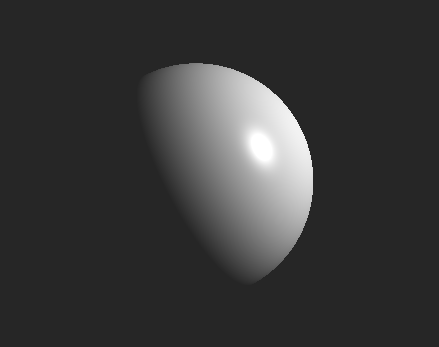
\includegraphics[width=0.51\textwidth]{./img/simplesphere.png}
\caption*{\label{fig:simplesphere}A simple ray marched sphere. \hyperref[sec:beginnings]{Back to section.}}
\end{figure}

\begin{figure}[htb]
\centering
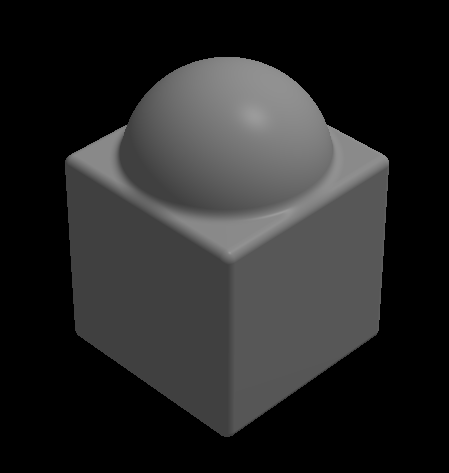
\includegraphics[width=0.51\textwidth]{./img/union.png}
\caption*{\label{fig:union}The union between a sphere and a cube. \hyperref[sec:creatingascene]{Back to section.}}
\end{figure}

\begin{figure}[htb]
\centering
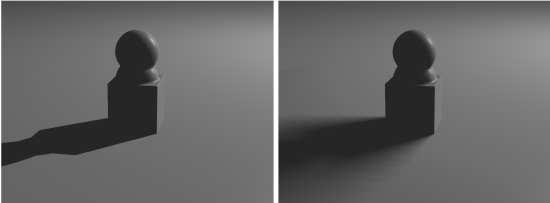
\includegraphics[width=0.99\textwidth]{./img/penumbra.png}
\caption*{\label{fig:penumbra}Penumbra shadowing in action. The left image has a \verb~k~-value of only 2, while the right image has a value of 128. \hyperref[sec:shadows]{Back to section.}}
\end{figure}

\begin{figure}[htb]
\centering
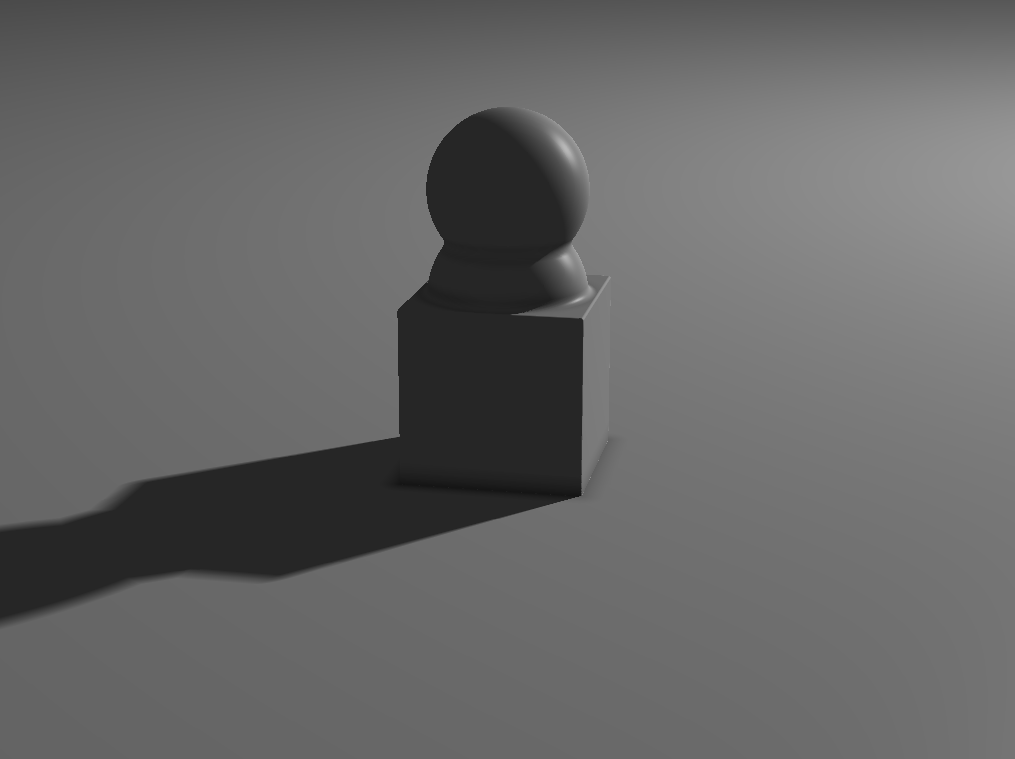
\includegraphics[width=0.99\textwidth]{./img/ao.png}
\caption*{\label{fig:ao}Ambient occlusion. Notice how some edges of the box are occluded by the floor. \hyperref[sec:ao]{Back to section}.}
\end{figure}

\begin{figure}[htb]
\centering
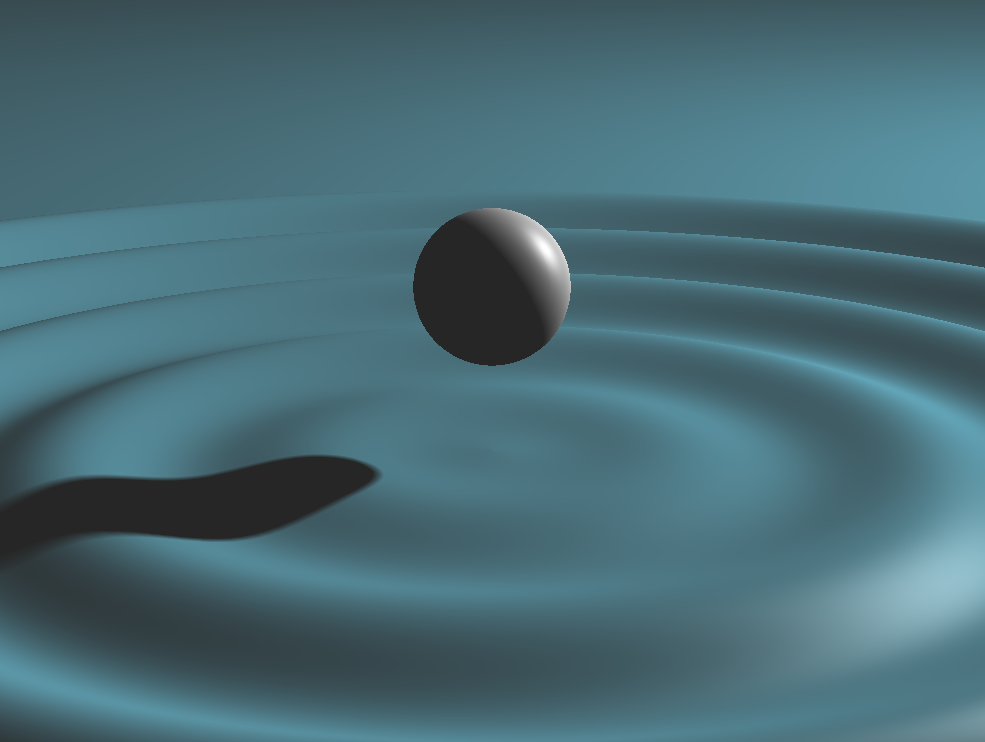
\includegraphics[width=0.99\textwidth]{./img/simplewater.png}
\caption*{\label{fig:simplewater}Very simple water shader in action, a gif can be found here: \url{http://folk.ntnu.no/thomaav/graphics/simplewater.gif}. \hyperref[sec:water]{Back to section}.}
\end{figure}

\begin{figure}[htb]
\centering
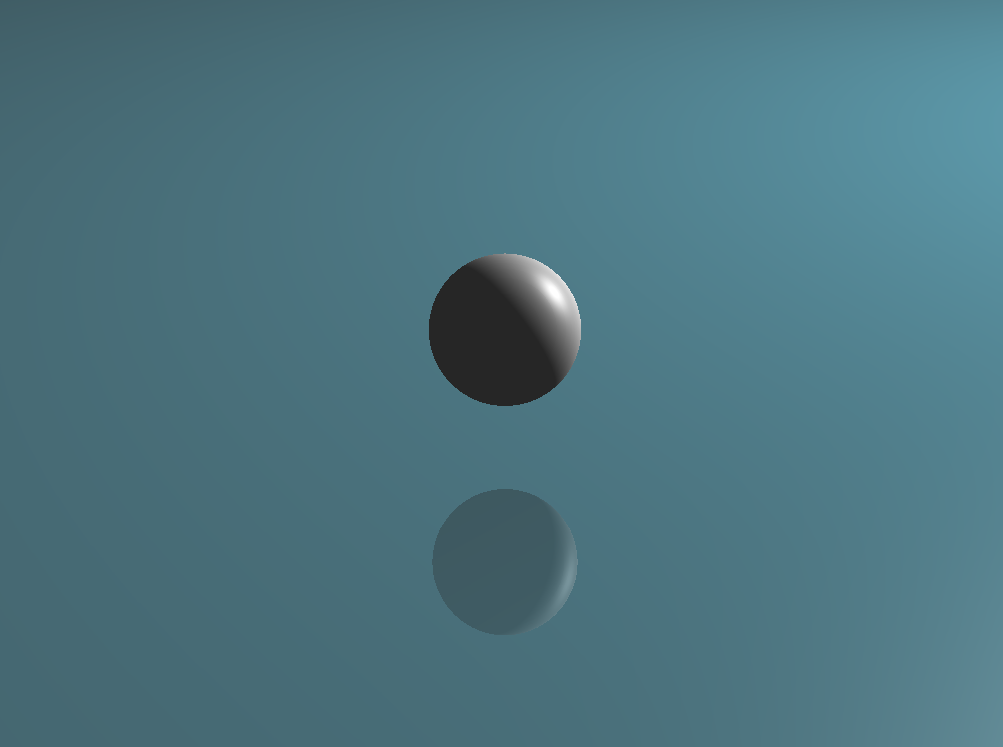
\includegraphics[width=0.99\textwidth]{./img/reflection.png}
\caption*{\label{fig:reflection}Reflection on the water surface, gif found at: \url{http://folk.ntnu.no/thomaav/graphics/reflection.gif}. \hyperref[sec:water]{Back to section}.}
\end{figure}

\begin{figure}[htb]
\centering
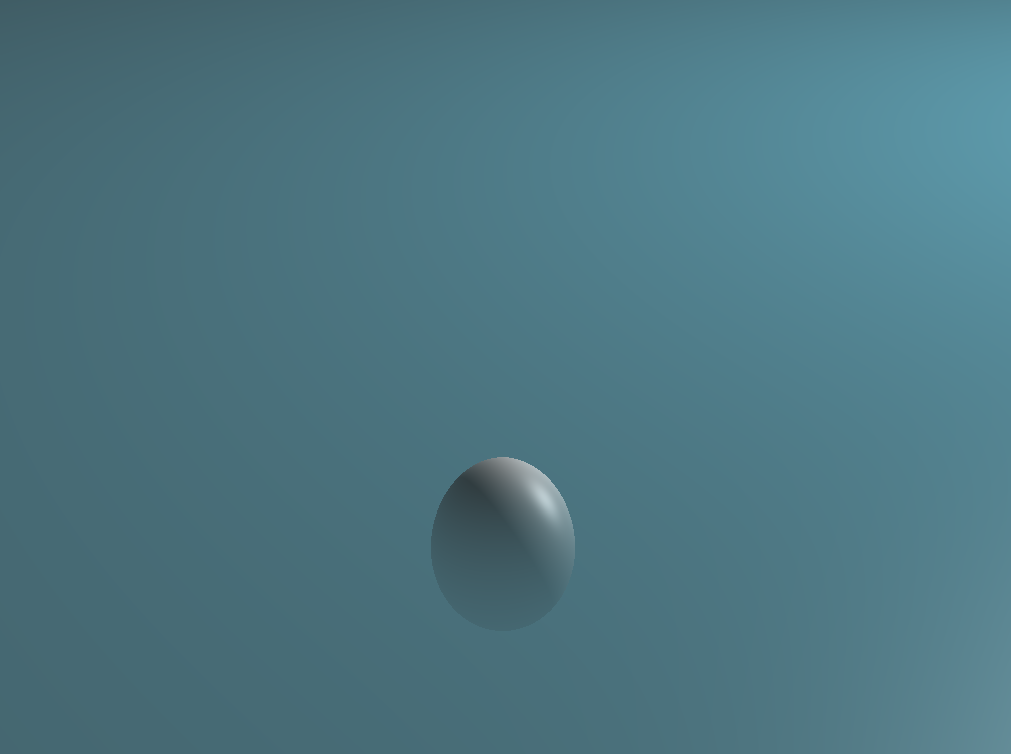
\includegraphics[width=0.99\textwidth]{./img/refraction.png}
\caption*{\label{fig:refraction}Refractive water surface. \url{http://folk.ntnu.no/thomaav/graphics/refraction.gif}. \hyperref[sec:water]{Back to section}.}
\end{figure}

\begin{figure}[htb]
\centering
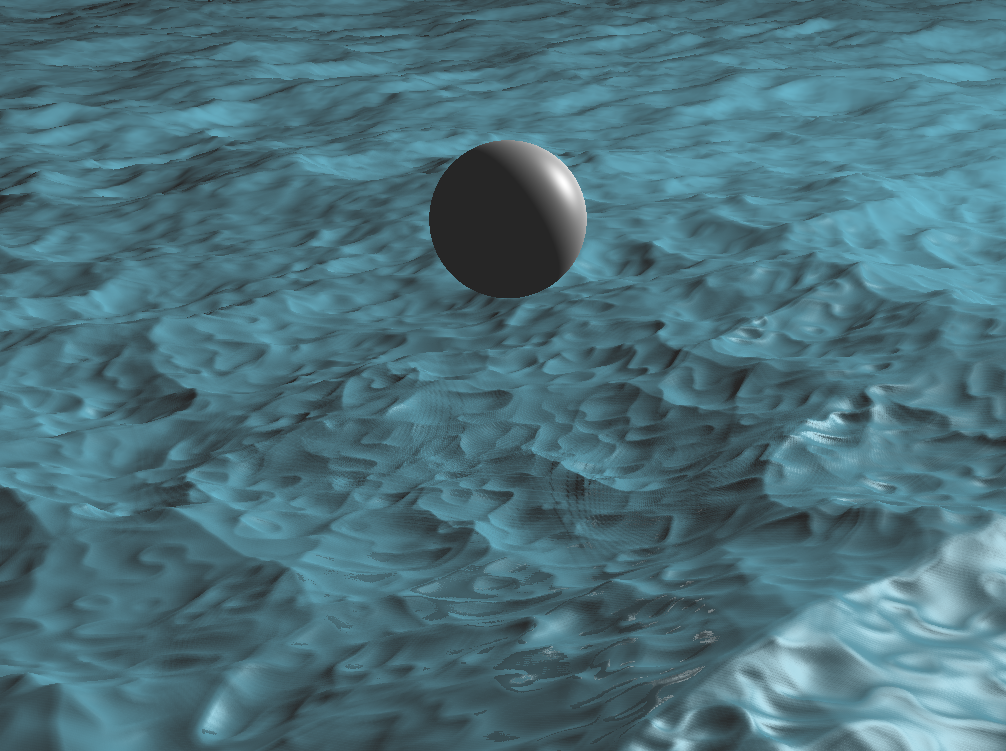
\includegraphics[width=0.99\textwidth]{./img/noise.png}
\caption*{\label{fig:noise}Water surface that is displaced with fBm. \url{http://folk.ntnu.no/thomaav/graphics/noise.gif}. \hyperref[sec:realisticwaves]{Back to section}.}
\end{figure}

\begin{figure}[htb]
\centering
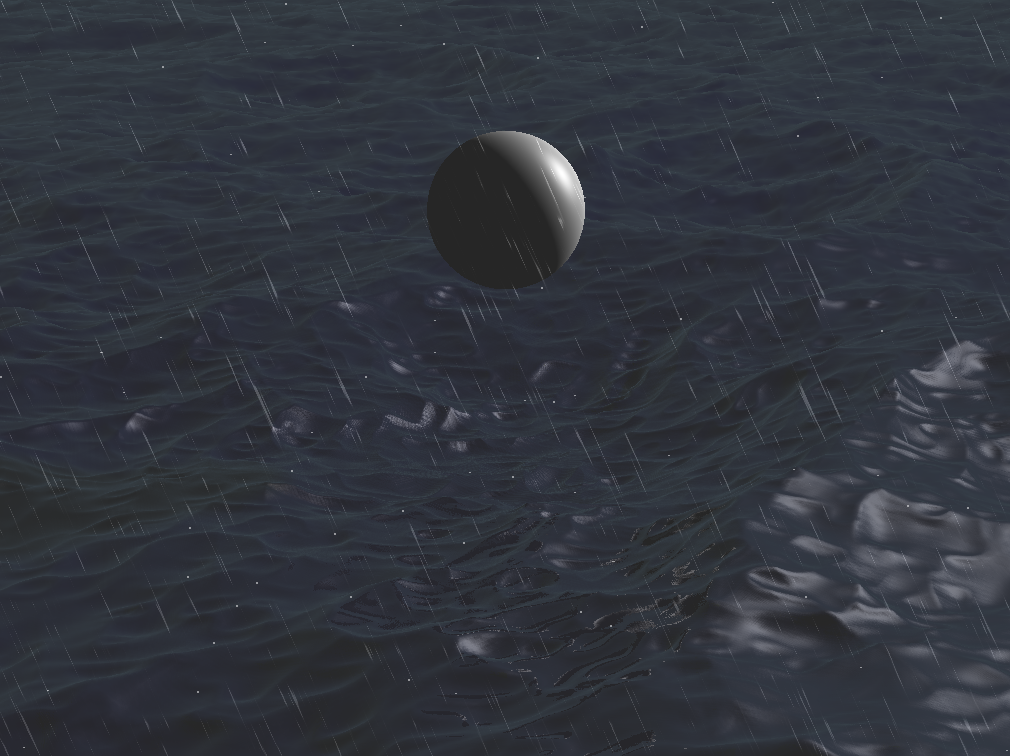
\includegraphics[width=0.99\textwidth]{./img/okwater.png}
\caption*{\label{fig:okwater}More realistic coloring of the water. \url{http://folk.ntnu.no/thomaav/graphics/okwater.gif}. \hyperref[sec:realisticcolor]{Back to section}.}
\end{figure}

\begin{figure}[htb]
\centering
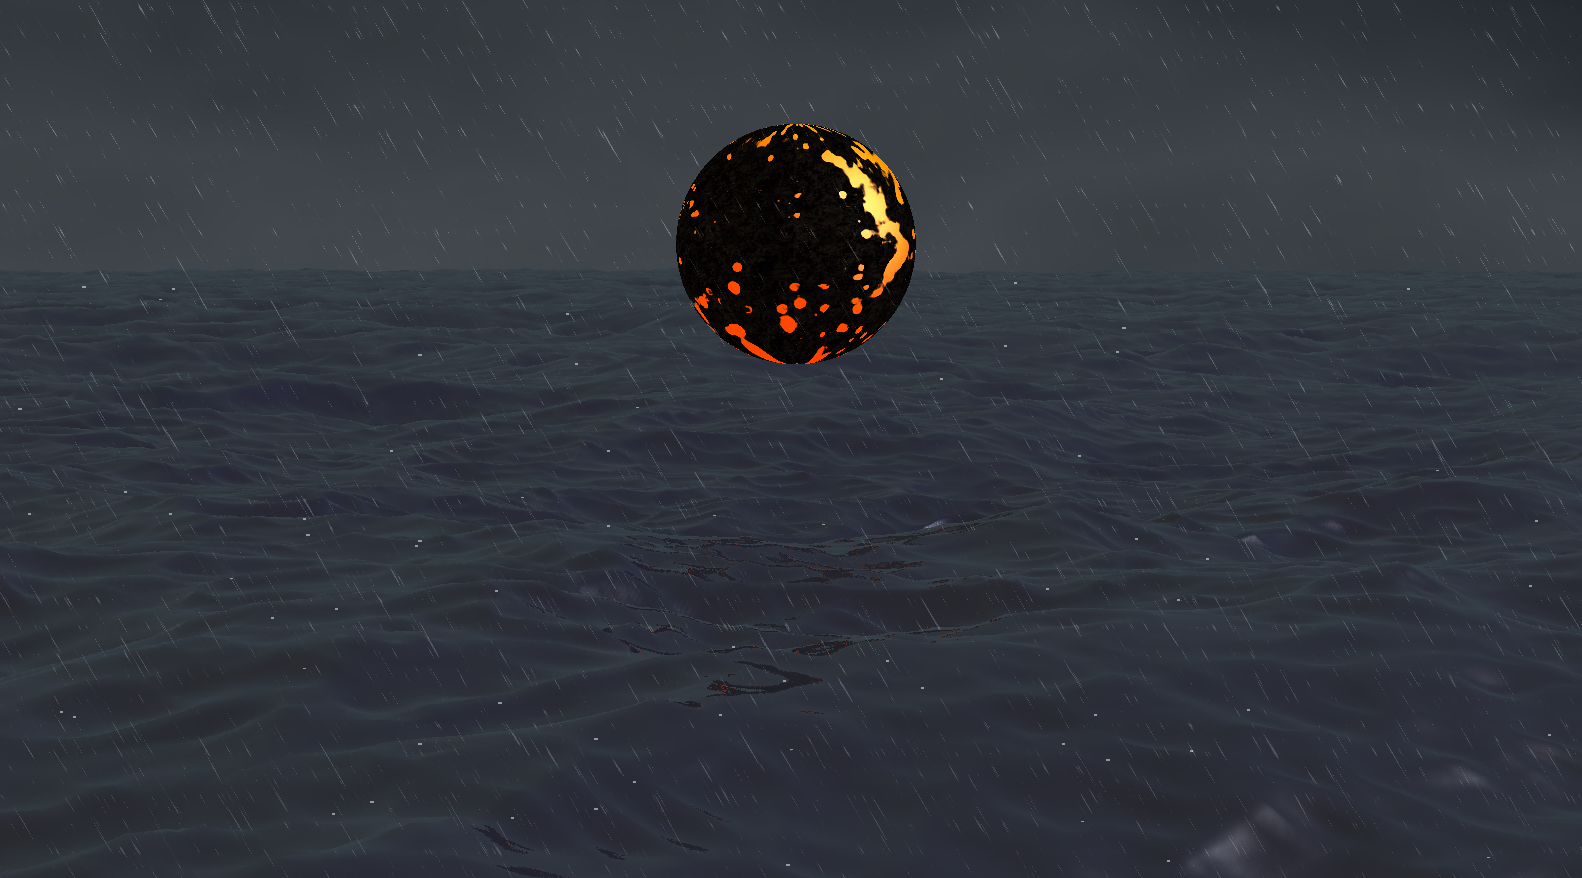
\includegraphics[width=0.99\textwidth]{./img/improvements.png}
\caption*{\label{fig:improvements}Further improvements on the scene. Includes procedurally texturing the sphere and adding clouds and lightning. \hyperref[sec:furtherimprovements]{Back to section}.}
\end{figure}

\begin{figure}[htb]
\centering
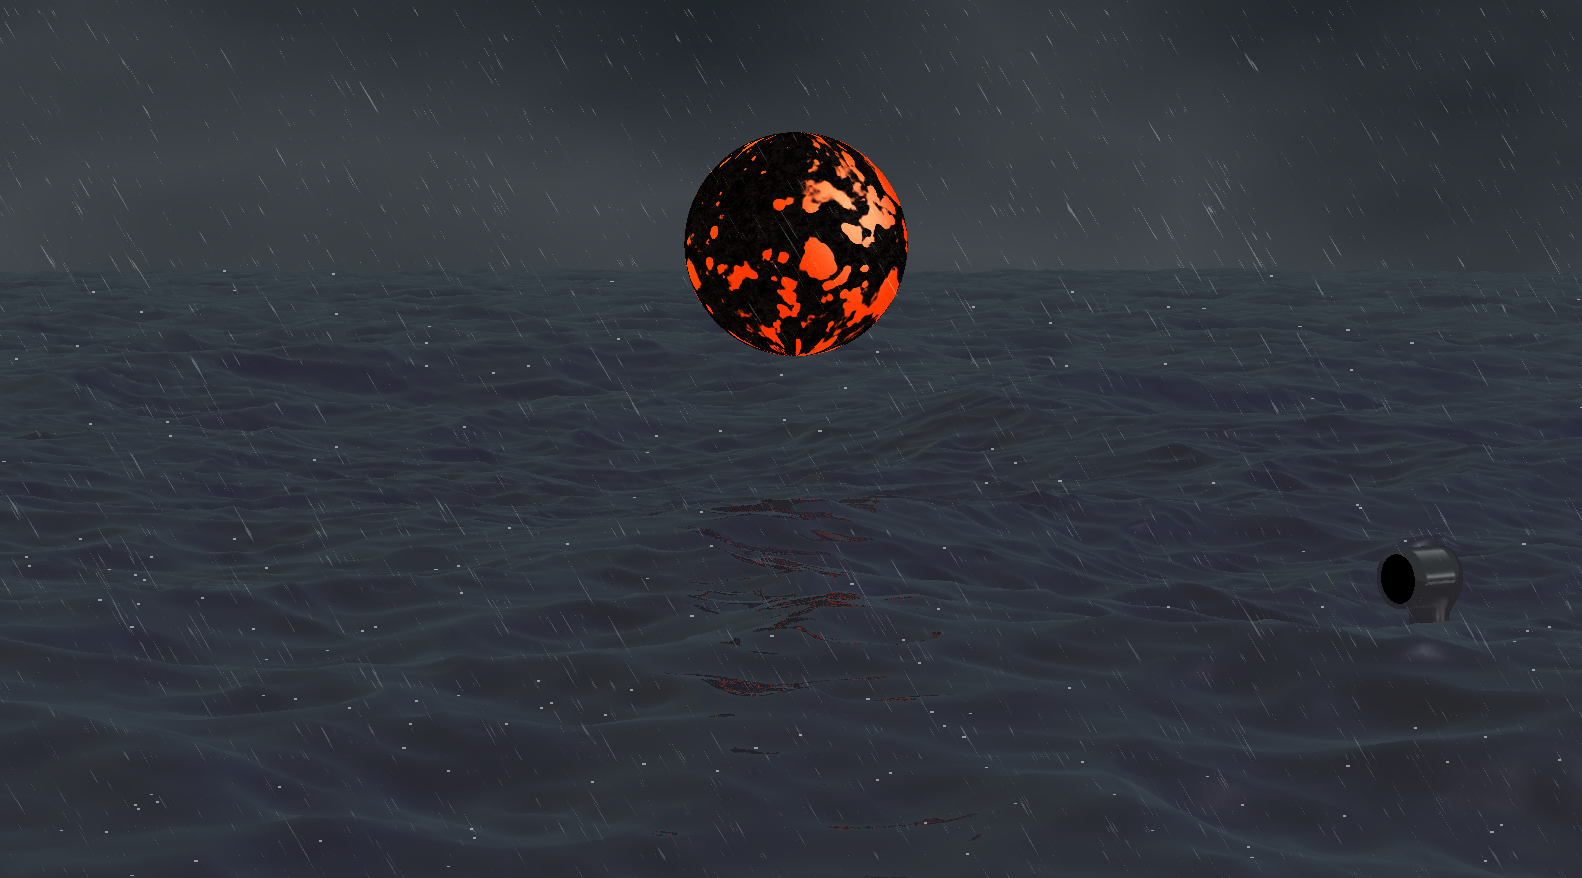
\includegraphics[width=0.99\textwidth]{./img/finalscene.png}
\caption*{\label{fig:finalscene}The final scene -- with the periscope visible in the lower right. The video is found at \url{https://www.youtube.com/watch?v=hDzagq61y1U} or \url{http://folk.ntnu.no/thomaav/graphics/shader.mp4}. \hyperref[sec:periscope]{Back to section}.}
\end{figure}
% Emacs 25.2.2 (Org mode 8.2.10)
\end{document}
